\section{实验}
\label{sec:experiment}

这一章节将会利用上一章介绍的两种目标跟踪方法在两段视频序列上进行实验,并对其实现效果、实时性进行展示和分析。
\twocolumn[{%
\renewcommand\twocolumn[1][]{#1}%
\noindent\begin{minipage}{\linewidth} 
 	\begin{center}
 	\vspace{0.3cm}
 	\captionsetup{font=small}
 	\begin{tabular}{@{}c@{}c@{}c@{}c@{}}
	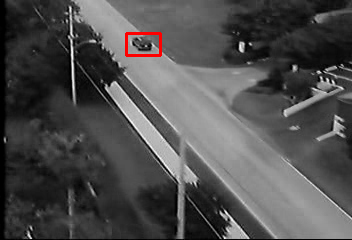
\includegraphics[width=0.25\linewidth]{fig3_a} &
 	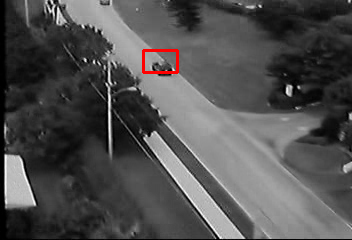
\includegraphics[width=0.25\linewidth]{fig3_b} &
 	 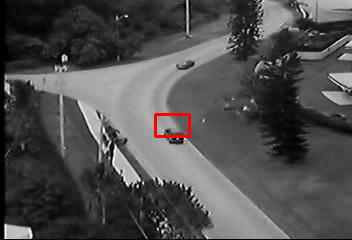
\includegraphics[width=0.25\linewidth]{fig3_c} &
    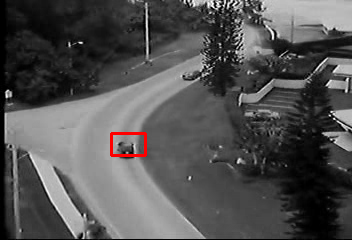
\includegraphics[width=0.25\linewidth]{fig3_d} \vspace{-1mm}\\
    {\small (a)} &  {\small (b)}  &  {\small (c)} &  {\small (d)} \\
    \end{tabular}
	\captionof{figure}{\small 在 Car\_Data 视频序列上实现基于 Mean Shift (均值漂移)目标跟踪: (a) 第一帧(手工标定目标初始位置), (b) 第十三帧, (c) 第六十八帧, and (d) 第一百帧.}
	\label{fig:car_result}
	\end{center}
	\vspace{0.5cm}
\end{minipage}
}]

\subsection{基于均值漂移的目标跟踪}

本文在 Car\_Data 视频序列上实现基于 Mean Shift (均值漂移)目标跟踪,待跟踪的目标为场景中的车辆,初始目标位置标定需手工标定\footnote{本文所进行的实验假设视频序列中目标尺度没有很大变化,故在实现算法中只考虑单一尺度,即首帧中的目标大小。
},后续帧中的目标位置需通过均值漂移方法得到。实验结果如图 \ref{fig:car_result} 所示,可以看到,在整个视频序列上,基于均值漂移的目标跟踪表现较好,可以比较准确地对场景中的车辆进行跟踪,仅仅在部分帧中,目标框的绘制与实际目标位置有所偏移。但其并不一定有如此良好的性能表现,与初始目标位置的标定(如目标框大小)有关,如图 \ref{fig:compare} 所示,在初始目标位置的标定发生改变后,在直线道路上跟踪效果依旧比较理想,但在弯道上目标框的绘制发生大幅度偏移,更甚至跟踪到另一辆车辆。这也印证了 Mean Shift 依赖对目标的描述而又缺乏必要的模板更新等原因,致使其对边缘遮挡、目标旋转、变形和背景运动不敏感。

\begin{figure}[!ht]
  \centering
  \begin{minipage}[b]{\linewidth} 
  \subfloat[]{
    \begin{minipage}[b]{0.31\linewidth} 
      \centering
      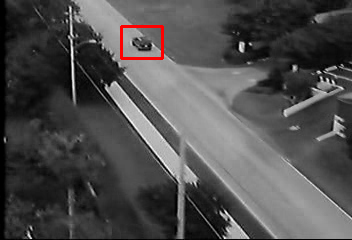
\includegraphics[width=\linewidth]{fig4_a}
       \end{minipage}
  }
  \subfloat[]{
    \begin{minipage}[b]{0.31\linewidth} 
      \centering
      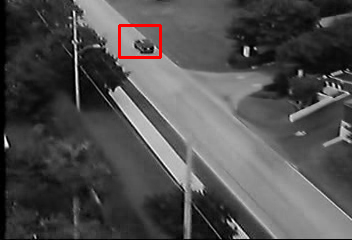
\includegraphics[width=\linewidth]{fig4_b}
       \end{minipage}
  }
\subfloat[]{
    \begin{minipage}[b]{0.31\linewidth} 
      \centering
      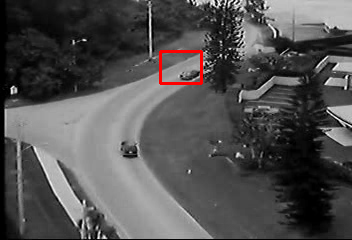
\includegraphics[width=\linewidth]{fig4_c}
       \end{minipage}
  }

  \end{minipage}
  \vfill
  \caption{在 Car\_Data 视频序列上实现基于 Mean Shift (均值漂移)目标跟踪: (a) 第一帧(手工标定目标初始位置), (b) 第二帧, and (c) 第九十七帧.}
  \label{fig:compare}
\end{figure}

\subsection{基于分类思想的目标跟踪}

\begin{figure}[!ht]
  \centering
  \begin{minipage}[b]{\linewidth} 
  \subfloat[]{
    \begin{minipage}[b]{0.23\linewidth} 
      \centering
      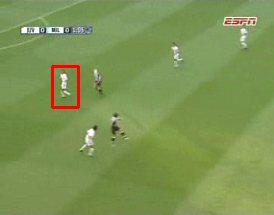
\includegraphics[width=\linewidth]{fig5_a1}\vspace{2pt}
      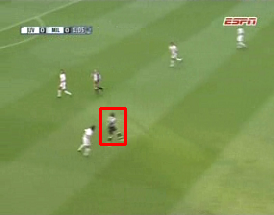
\includegraphics[width=\linewidth]{fig5_a2}
       \end{minipage}
  }
  \subfloat[]{
    \begin{minipage}[b]{0.23\linewidth} 
      \centering
      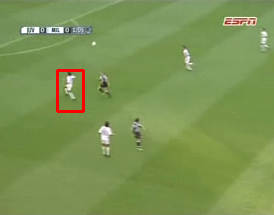
\includegraphics[width=\linewidth]{fig5_b1}\vspace{2pt}
      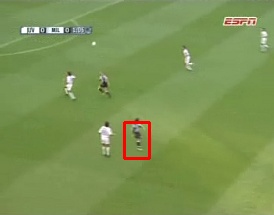
\includegraphics[width=\linewidth]{fig5_b2}
       \end{minipage}
  }
\subfloat[]{
    \begin{minipage}[b]{0.23\linewidth} 
      \centering
      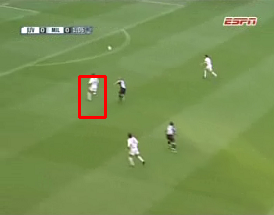
\includegraphics[width=\linewidth]{fig5_c1}\vspace{2pt}
      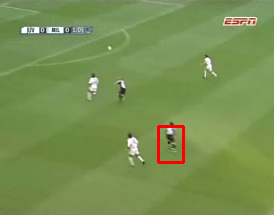
\includegraphics[width=\linewidth]{fig5_c2}
       \end{minipage}
  }
  \subfloat[]{
    \begin{minipage}[b]{0.23\linewidth} 
      \centering
      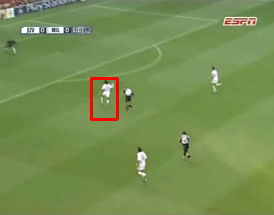
\includegraphics[width=\linewidth]{fig5_d1}\vspace{2pt}
      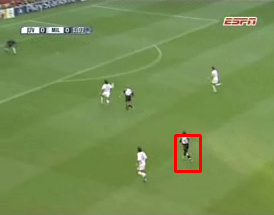
\includegraphics[width=\linewidth]{fig5_d2}
       \end{minipage}
  }

  \end{minipage}
  \vfill
  \caption{在 Football 视频序列上实现基于分类思想的目标跟踪: 上:对左上角足球运动员进行跟踪;下:对右下角足球运动员进行跟踪. (a) 第一帧(手工标定目标初始位置), (b) 第十帧, (c) 第二十帧, and (d) 第三十帧.}
  \label{fig:football_result}
\end{figure}


\begin{figure}[!ht]
  \centering
  \begin{minipage}[b]{\linewidth} 
  \subfloat[]{
    \begin{minipage}[b]{0.31\linewidth} 
      \centering
      
\includegraphics[width=\linewidth]{fig6_a}
       \end{minipage}
  }
  \subfloat[]{
    \begin{minipage}[b]{0.31\linewidth} 
      \centering
      
\includegraphics[width=\linewidth]{fig6_b}
       \end{minipage}
  }
\subfloat[]{
    \begin{minipage}[b]{0.31\linewidth} 
      \centering
      
\includegraphics[width=\linewidth]{fig6_c}
       \end{minipage}
  }

  \end{minipage}
  \vfill
  \caption{在 Football 视频序列上实现基于分类思想的目标跟踪获得的置信图: (a) 第二帧, (b) 第十帧, and (c) 第二十七帧.}
  \label{fig:confidence}
\end{figure}

本文在 Football 视频序列上实现基于分类思想的目标跟踪,分类器采用二分类的支持向量机,并设置分类器的个数为5,待跟踪的目标为场景中的某个运动员,初始目标位置标定需手工标定,后续帧中的目标位置需通过在线分类器得到。实验结果如图 \ref{fig:football_result} 所示,可以看到,在部分视频序列上,基于分类思想的的目标跟踪表现较为理想,基本可以在复杂的环境中准确地目标进行跟踪,即使目标的形状发生了改变。但由于训练数据的标注较为粗糙,将目标框内的所有像素都标注为目标,从而导致训练得到一个好的分类器更加困难,反映到目标跟踪上为随着视频序列的演进,目标的跟踪逐渐偏移。除此以外,也与目标的尺度变化有一定的关系,后续改进可以在不同尺度的图片上对模型进行训练并将不同尺度的预测结果进行融合。基于分类思想的目标跟踪在分类得到的置信图上利用 Mean Shift 算法对目标位置进行预测,如图 \ref{fig:confidence} 所示,置信图与真实情况基本相符,整体跟踪效果比较好,在出现遮挡的情况下仍能够实现较好的跟踪,没有丢失目标。


\begin{table}[!htbp]
\caption{不同跟踪方法的实时性比较}
\centering
\label{tab:measurement}
\setlength{\tabcolsep}{7.5mm}{
\begin{tabular}{c|c|c}
\hline
& 均值漂移 & Adaboost \\
\hline
单张耗时(秒) & 0.019 & 3.26 \\
处理帧数(fps)& 51.36 & 0.3067\\
\hline
\end{tabular}
}
\end{table}

\newpage
对于算法的实时性,如表 \ref{tab:measurement} 所示,基于均值漂移的目标跟踪方法计算量不大,在目标区域已知的情况下完全可以做到实时跟踪;而对于基于分类思想的目标跟踪方法,虽然采用了在线更新的策略,且算法简单,但由于算法的实现采样点过密,计算量相对较大,实时性较差。尤其是对于第一帧要对多个若分类器进行初始化训练,所需时间更长。